\section{Tracing}

\subsection{Software Architecture and Methodologies}

\begin{frame}[fragile]{Tracing}
    \begin{block}{Tecnologie}
        \begin{itemize}
            \item OpenTelemetry (OTLP)
            \item Jaeger
        \end{itemize}
    \end{block}
    \begin{block}{Estensioni}
        \begin{minted}{bash}
<dependency>
    <groupId>io.quarkus</groupId>
    <artifactId>quarkus-opentelemetry</artifactId>
</dependency>
        \end{minted}
    \end{block}
\end{frame}

\begin{frame}[fragile]{Tracing}
    \begin{block}{Jaeger: configurazione}
        \begin{minted}[fontsize=\footnotesize]{bash}
quarkus.otel.service.name=inventory-service
quarkus.otel.exporter.otlp.endpoint=
    =http://jaeger-collector:4317
quarkus.otel.traces.sampler=always_on
        \end{minted}
    \end{block}
    \begin{block}{Jaeger: Helm deployment}
        \begin{minted}[fontsize=\footnotesize]{bash}
helm install jaeger jaegertracing/jaeger \
    --set allInOne.enabled=true \
    --set agent.enabled=false \
    --set collector.enabled=false \
    --set query.enabled=false \
    --set provisionDataStore.cassandra=false \
    --set storage.type=memory
        \end{minted}
    \end{block}
\end{frame}

\begin{frame}{Tracing}
    \begin{columns}
        \begin{column}{.4\textwidth}
            \centering
            \begin{block}{Use case}
                Utente che effettua una prenotazione.
            \end{block}
        \end{column}
        \begin{column}{.6\textwidth}
            \centering
            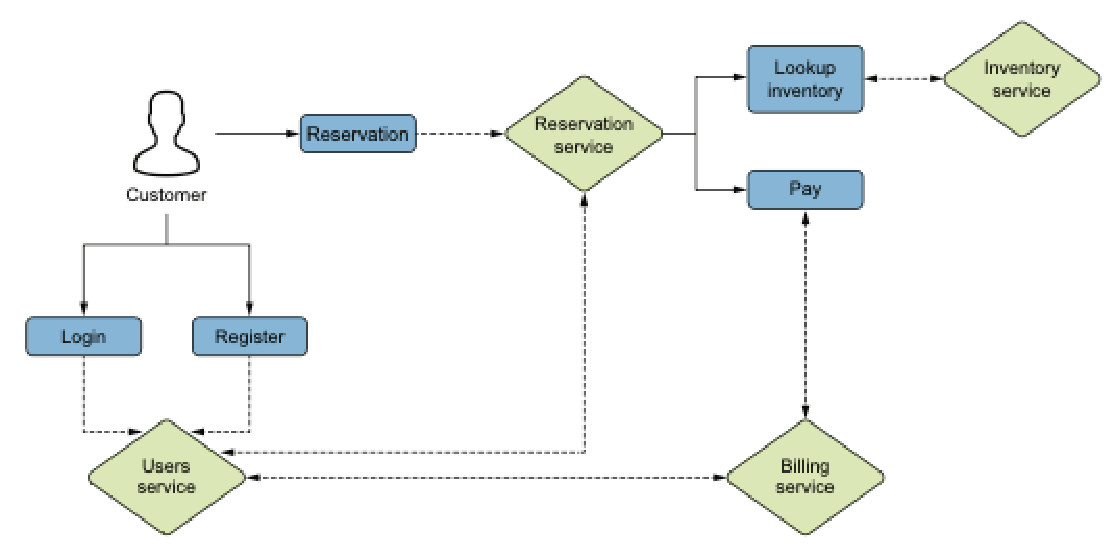
\includegraphics[width=.7\textwidth]{images/4-tracing/use cases.pdf}
        \end{column}
    \end{columns}
    \centering
    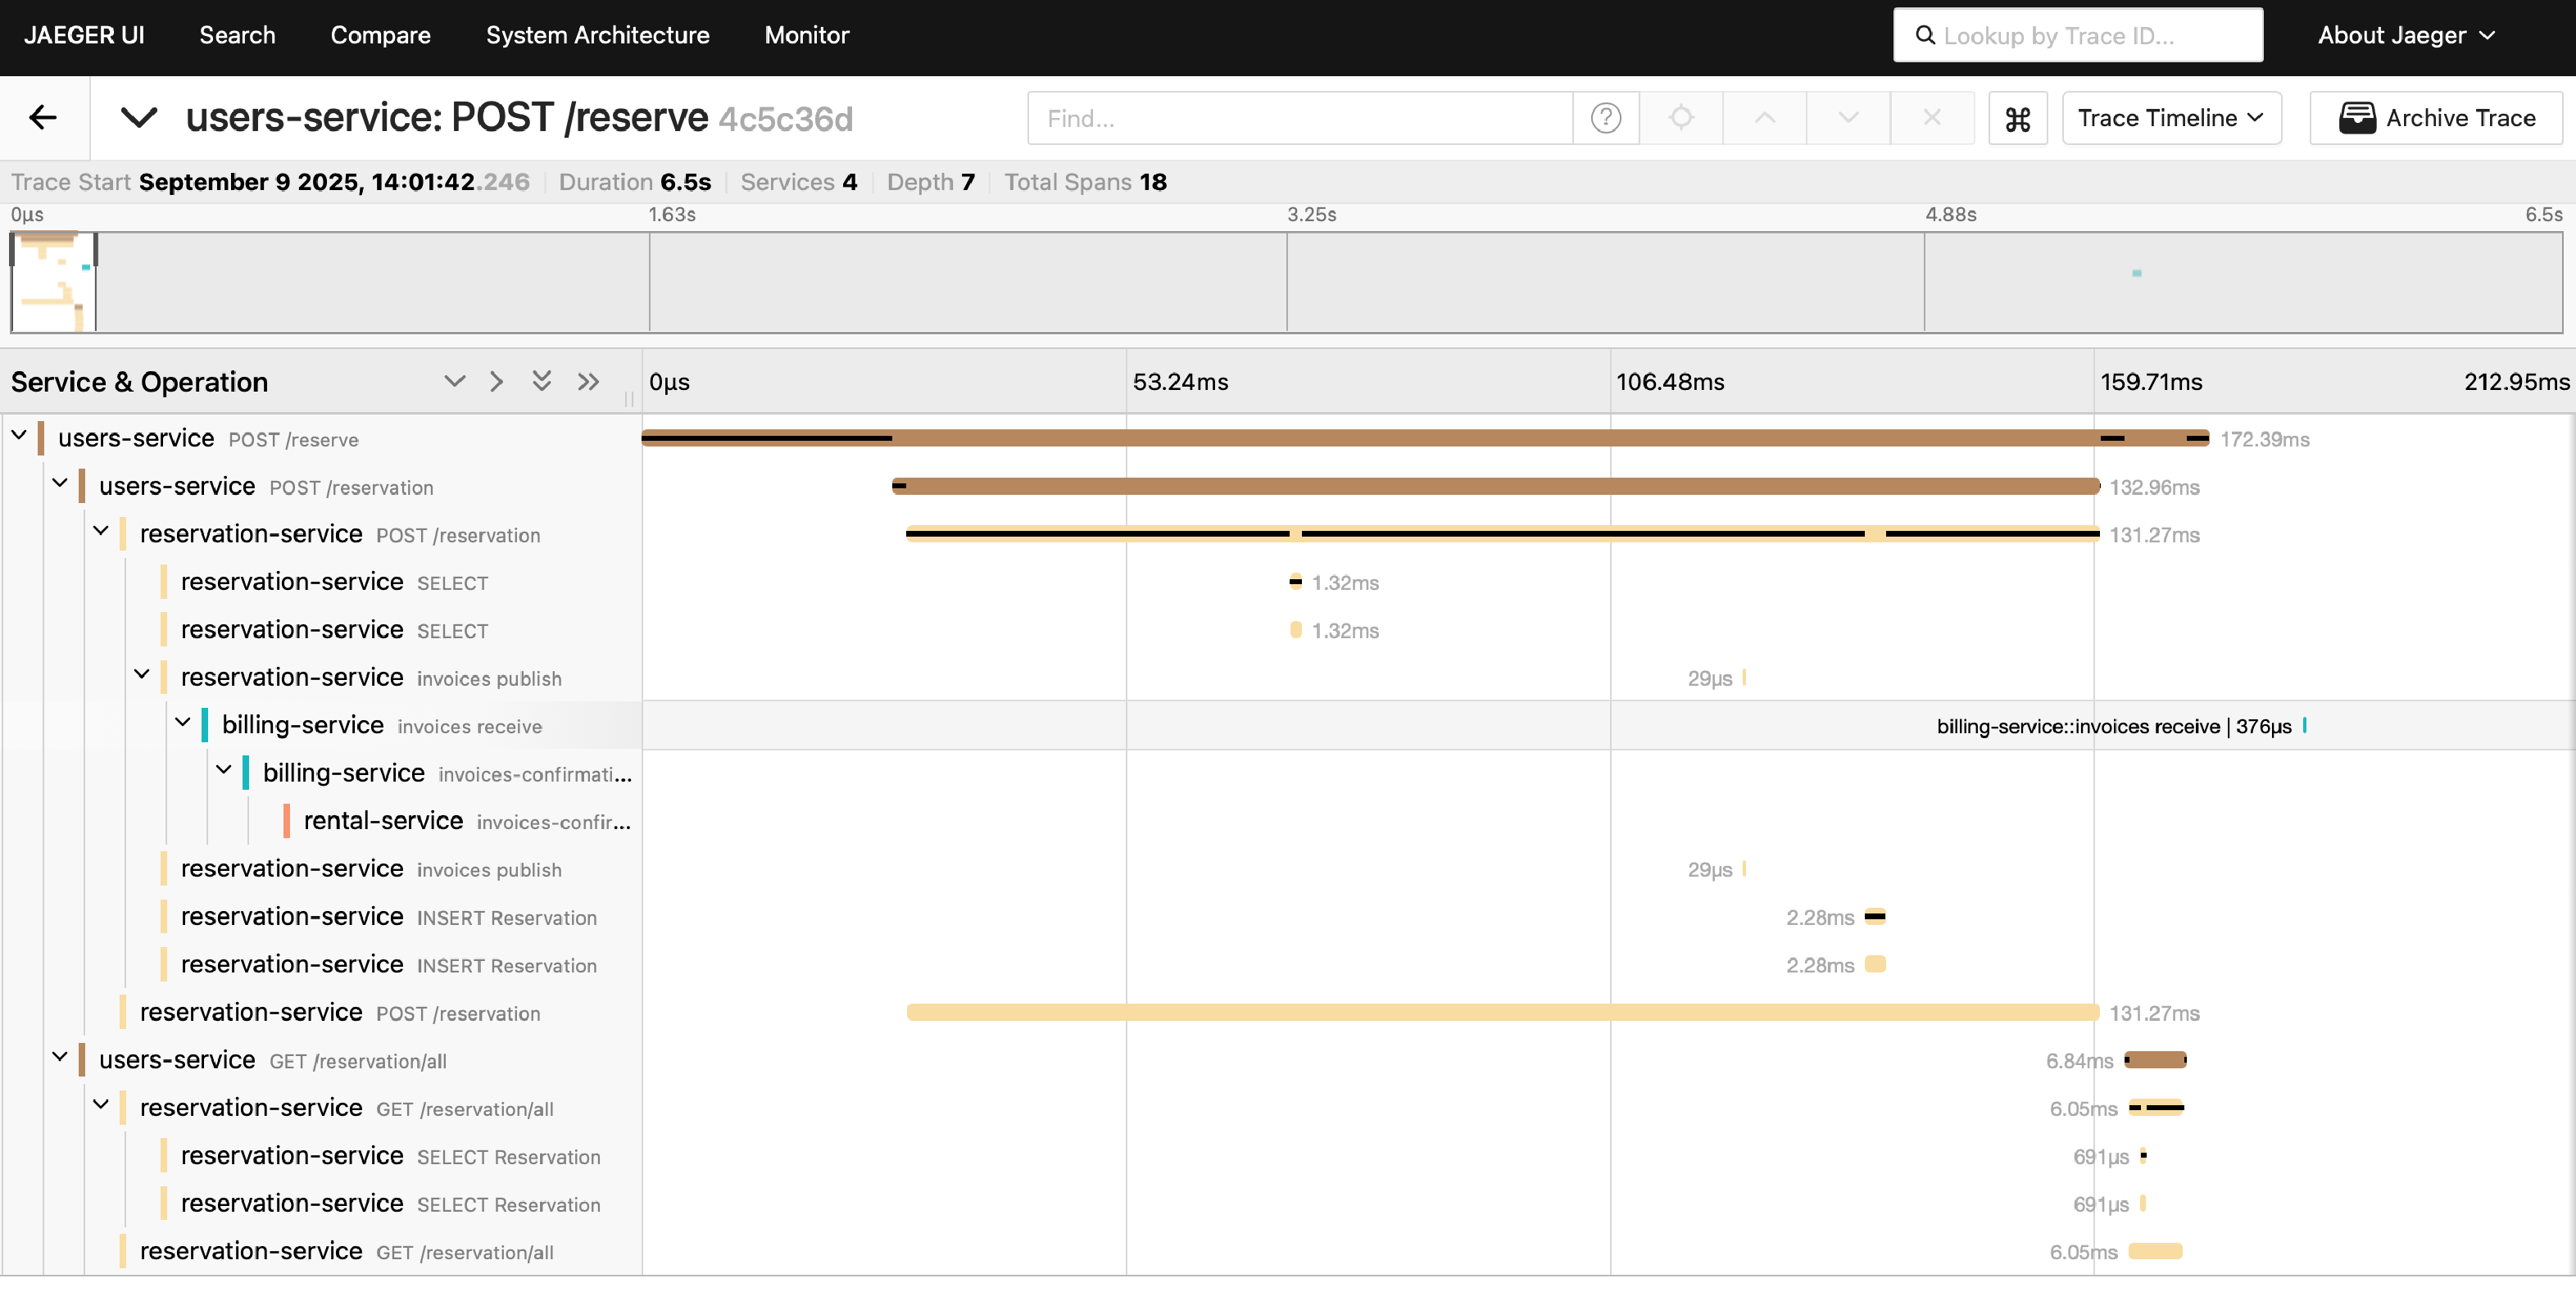
\includegraphics[width=.8\textwidth]{images/4-tracing/jaeger use case.pdf}
\end{frame}